\chapter{Metodoloxía e planificación}
\label{chap:Metodoloxía e planificación}
\lettrine{N}{esta} sección explícase a metodoloxía de traballo empregada para o desenvolvemento do proxecto, así como a planificación do mesmo.
 Ademais, descríbense os recursos utilizados e faise unha estimación dos custos asociados ao proxecto.

\section{Metodoloxía do desenrolo}
\label{sec:Metodoloxía do desenrolo}

Ao ser un proxecto de investigación, a metodoloxía de traballo máis adecuada é unha metodoloxía iterativa e incremental, que permite poder adaptarse aos cambios que van xurdindo durante o desenrolo do proxecto.
Esta metodoloxía permite obter un artefacto funcional ao final de cada iteración, o que permite obter retroalimentación constante sobre o desenrolo do proxecto.
Cada iteración comeza cunha análise do que se quere conseguir, seguida das fases de deseño e codificación, e remata cunha fase de testeo do produto desenvolvido.

\section{Planificación do proxecto}
\label{sec:Planificación do proxecto}
O proxecto inicialmente divídese nas seguintes fases principais:

\begin{itemize}
    \item \textbf{Revisión do estado da arte:}
    \begin{itemize}
        \item Estudo do dominio biolóxico: características das imaxes oftalmolóxicas, a súa importancia e aplicacións.
        \item Análise de traballos relacionados con IDIR, representacións implícitas e segmentación de imaxes oftalmolóxicas mediante redes neuronais.
    \end{itemize}
    Esta fase estimouse en aproximadamente 3 semanas de traballo, dada a necesidade de familiarizarse co contexto e identificar solucións previas relevantes.

    \item \textbf{Análise do traballo base:}
    \begin{itemize}
        \item Estudo en profundidade do código orixinal de IDIR.
        \item Replicación dos resultados orixinais para verificar o funcionamento correcto.
    \end{itemize}
    O esforzo estimado para esta tarefa foi de 2 semanas, considerando a análise do código e a posta en marcha do entorno.

    \item \textbf{Adaptación ao novo dominio:}
    \begin{itemize}
        \item Modificación da arquitectura para traballar con imaxes 2D en lugar de 4D.
        \item Implementación das adaptacións necesarias para imaxes oftalmolóxicas.
    \end{itemize}
    Esta etapa estímase unha duración de 5 semanas, debido á complexidade das modificacións e probas necesarias.

    \item \textbf{Avaliación e experimentación:}
    \begin{itemize}
        \item Deseño dunha metodoloxía de avaliación específica para o novo dominio.
        \item Realización de múltiples experimentos para optimizar o rendemento.
        \item Validación da efectividade en imaxes oftalmolóxicas.
    \end{itemize}
    Estímase un esforzo de 8 semanas, repartidas entre o deseño experimental, execución e análise dos resultados dos distintos experimentos.

    \item \textbf{Documentación:}
    \begin{itemize}
        \item Redacción da memoria final do proxecto.
        \item Análise e presentación dos resultados obtidos.
    \end{itemize}
    Para a documentación reserváronse 2 semanas, incluíndo a redacción, revisión e preparación dos anexos. A memoria será redactada ao longo de todo o proceso, pero nesta fase final revisaráse e completarase.
\end{itemize}

En total, estímase unha duración de 20 semanas para o proxecto, repartidas entre as distintas fases.
Na figura \ref{fig:planificacion_proxecto} móstrase o diagrama de Gantt que resume a planificación do proxecto, indicando as fases principais e a súa duración estimada.

\begin{figure}[tbp]
    \centering
    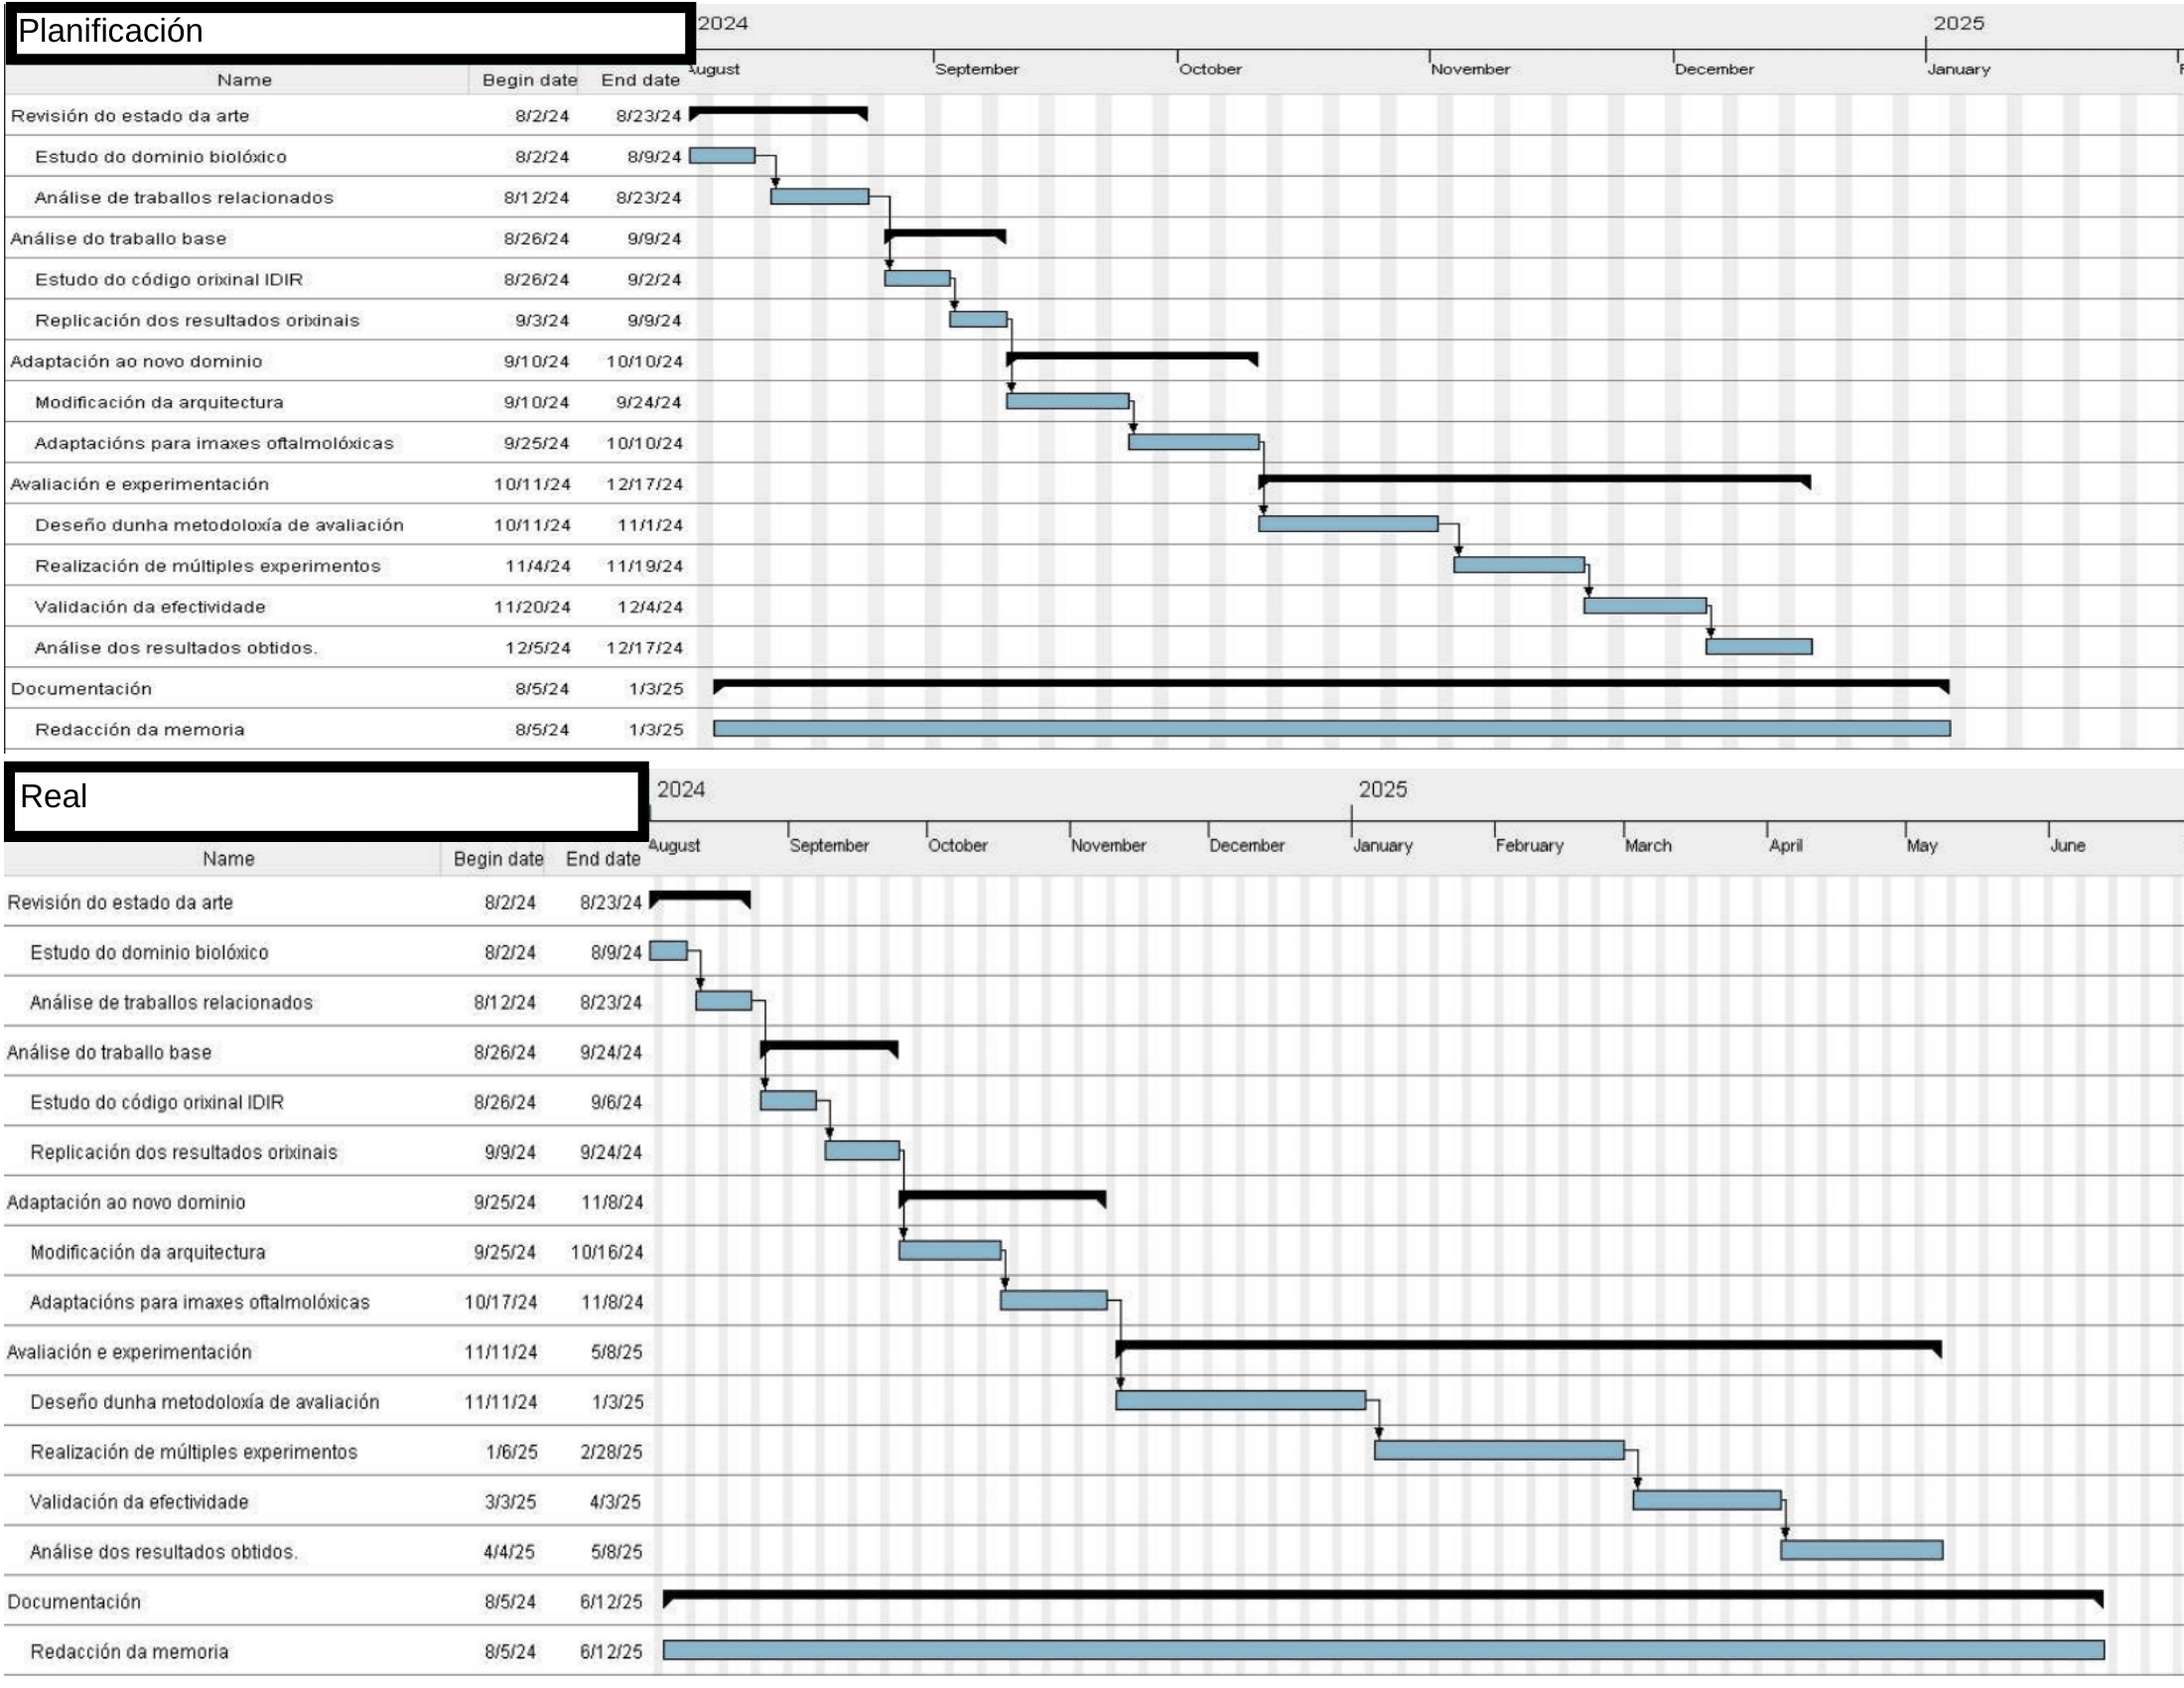
\includegraphics[height=1\textwidth, angle=90]{imaxes/gants-1.png}
    \caption{Diagramas de Gantt da planificación do proxecto e duración real de cada fase}
    \label{fig:planificacion_proxecto}
\end{figure}

\section{Recursos utilizados}
\label{sec:Recursos utilizados}

\subsection{Software}
\label{subsec:Software}

Xa que parte do traballo consiste en adaptar un traballo previo, 
decidíuse empregar moito do mesmo software ca o traballo orixinal para facilitar a implementación e reproducibilidade.
O mais relevante é PyTorch, unha librería de código aberto para Python que facilita o desenrolo de redes neuronais. Utilizáronse as versións de Python 3.12.3 e CUDA 12.2. Tamén se empregan librerías de apoio como NumPy (para traballar con matrices), Matplotlib (visualización), OpenCV ou scikit-learn (manexo de imaxes).

Outro software empregado inclúe VSCode (IDE), Git (control de versións) e LaTeX (redacción de memoria).

\subsection{Hardware}
\label{subsec:Hardware}

O proxecto foi desenrrolado nun ordenador portátil conectado por ssh a un servidor con GPU. 
Utilizáronse dous servidores diferentes, un montado por min\footnote{\url{https://blog.m19182.dev/writings/Building-my-Homelab}} e outro facilitado polo grupo de investigación VARPA (Visión Artificial y Reconocimiento de Patrones).

A gran parte dos experimentos foron realizado no primeiro, mais para poder executar o proxecto cas imaxes na súa resolución orixinal foi necesario empregar o segundo 
debido ás limitacións de memoria da GPU. Na táboa \ref{tab:comparativa_servidores} móstrase unha comparativa entre os servidores utilizados, indicando as principais características de hardware de cada un.

\begin{table}[tbp]
\centering
\begin{tabular}{|c|c|c|}
\hline
\textbf{Característica} & \textbf{Homelab} & \textbf{Servidor VARPA} \\ \hline
Procesador & AMD Ryzen 9 5950X&  AMD Ryzen Threadripper 3960X \\ \hline
GPU & NVIDIA RTX 3090 & NVIDIA RTX A6000  \\ \hline
\end{tabular}
\caption{Comparativa entre os servidores utilizados}
\label{tab:comparativa_servidores}
\end{table}


\subsection{Conxuntos de datos}
\label{subsec:Conxuntos de datos}
Para o desenrolo do proxecto empregáronse dous conxuntos de datos diferentes:

\begin{itemize}
    \item \textbf{RFMID:} 3200 imaxes de fondo de ollo en cor con resolución 1712x1712.
    \item \textbf{FIRE:} 134 pares de imaxes de retinas en cor, cun tamaño de 2912×2912 pixels
\end{itemize}

Estos son descritos en maior detalle na sección \ref{sec:Conxuntos de datos}.

\subsection{Estimación de custos}
\label{subsec:Estimación de custos}

Os custos do hardware son ignorados xa que xa estaba dispoñible antes da realización do proxecto.

Os custos dos recursos humanos calcúlanse para un estudante e dous titores, resultando nun custo estimado de 20.680€, IVE incluído. A táboa \ref{tab:estimacion_custos} mostra a estimación de custos dos recursos humanos desglosados, considerando un estudante a 20€/hora e titores a 35€/hora.

\begin{table}[h]
\centering
\begin{tabular}{|c|c|c|c|}
\hline
\textbf{Recurso} & \textbf{Custo por hora} & \textbf{Horas estimadas} & \textbf{Custo total} \\ \hline
Estudante & 20€ & 880h & 17.600€ \\ \hline
Titor 1 & 35€ & 44h & 1.540€ \\ \hline
Titor 2 & 35€ & 44h & 1.540€ \\ \hline
\end{tabular}
\caption{Estimación de custos dos recursos humanos (IVE incluído)}
\label{tab:estimacion_custos}
\end{table}

\section{Seguimento da planificación}
\label{sec:Seguimento da planificación}

A planificación do proxecto foi revisada periodicamente segundo as fases do proxecto, e para identificar desviacións respecto ao plan inicial.

Pese a que nas fases iniciais do proxecto se respectou a planificación, a fase de adaptación ao novo dominio e a fase de avaliación e experimentación sufriron retrasos significativos.

A fase de adaptación ao novo dominio requiriu máis tempo do esperado debido á complexidade das modificacións necesarias para adaptar o modelo a imaxes 2D, así como á necesidade de realizar múltiples probas para garantir o correcto funcionamento do modelo adaptado. A fase de avaliación tamén se viu afectada, xa que requiriu máis tempo do esperado para deseñar unha metodoloxía de avaliación adecuada. Finalmente, a fase de experimentación requiriu máis tempo do previsto, en parte debido aos malos resultados obtidos inicialmente, que obrigaron a revisar en profundidade o código e implementar novas probas para asegurar a correcta implementación.
En total, isto conlevou un retraso de aproximadamente 18 semanas respecto á planificación inicial.

A fase final de análise de resultados e redacción da memoria tamén se viu afectada, aínda que en menor medida, o que conlevou un retraso adicional de 2 semanas, resultando nunha duración total do proxecto de 40 semanas, fronte ás 20 semanas inicialmente previstas.

Na figura \ref{fig:planificacion_proxecto} móstrase o diagrama de Gantt actualizado, que reflicte a duración real de cada fase do proxecto.

\subsection{Estimación de custo real}
\label{subsec:Estimación de custo real}

A estimación de custo do proxecto foi de 20.680€, como se indicou na sección \ref{subsec:Estimación de custos}. Non obstante, debido aos retrasos no desenvolvemento do proxecto, o custo real aumentou de forma proporcional ao tempo extra empregado.

Dado que o proxecto se estendeu durante 20 semanas máis do previsto (o dobre da planificación inicial), o custo real estimado ascende a 41.360€ (IVE incluído).